\documentclass[border=10pt]{standalone}
\usepackage{pgfplots}
\usepgfplotslibrary{colormaps}
\pgfplotsset{compat=1.18}

\begin{document}
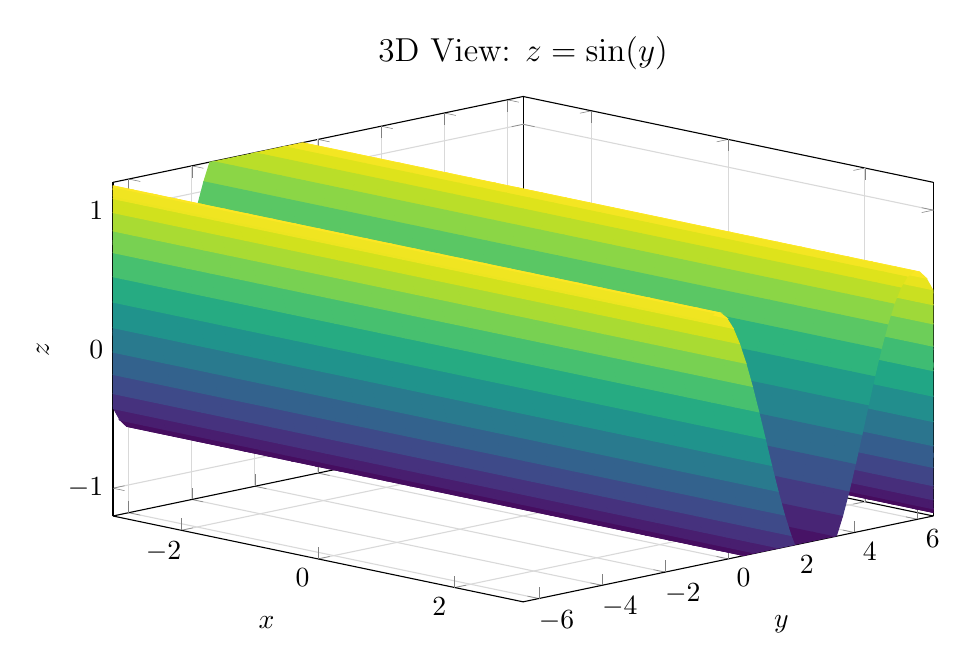
\begin{tikzpicture}
\begin{axis}[
    view={45}{20},
    xlabel={$x$},
    ylabel={$y$},
    zlabel={$z$},
    title={3D View: $z = \sin(y)$},
    title style={font=\large},
    width=12cm,
    height=8cm,
    colormap/viridis,
    grid=major,
    grid style={gray!30},
    xmin=-3, xmax=3,
    ymin=-6.5, ymax=6.5,
    zmin=-1.2, zmax=1.2,
    samples=30,
    samples y=50,
]
\addplot3[surf, shader=flat corner] {sin(deg(y))};
\end{axis}
\end{tikzpicture}
\end{document}